\chapter{Contesto teorico}
In questo capitolo si descrive il contesto di ricerca in cui si inserisce questo progetto di tesi, andando a descrivere lo stato dell'arte della simulazione delle masse (Sezione \ref{subsec:stato-dell-arte}) e l'approccio di ricerca in cui questo progetto di tesi si è reso necessario (Sezione \ref{subsec:approccio-gerarchico}).\\
Successivamente si fornisce una descrizione dell'ambiente NetLogo (Sezione \ref{sec:netlogo}) e dei Design Patterns (Sezione \ref{sec:builder} e \ref{sec:visitor}) che questo progetto usa al fine di una migliore comprensione e chiarezza dei concetti esposti nel Capitolo \ref{cap:sviluppo-progetto}.
\section{Simulazione delle masse}
\label{sec:simulazione-masse}
Come già accennato nell'introduzione, la simulazione delle masse è un ambito di ricerca che negli ultimi anni ha guadagnato molta rilevanza. Questo grazie a un miglioramento delle capacità computazionali e dei metodi utilizzati, ma anche a causa di eventi sociali sempre più frequenti e di dimensioni sempre maggiori. Quindi diventa sempre più importante la capacità di prevedere i movimenti delle masse in modo da garantire la sicurezza delle persone in ogni tipo di situazione.\\
Le criticità che rendono la modellazione delle masse un problema complesso sono le grandi dimensioni dei modelli e i comportamenti individuali, sia sociali che fisici, che devono essere presi in considerazione.\\
Descriviamo brevemente gli approcci più diffusi e riconosciuti per la simulazione delle masse per andare poi a soffermarci sull'approccio gerarchico in cui si inserisce questo progetto di tesi.
\subsection{Stato dell'arte}
\label{subsec:stato-dell-arte}
Nella modellazione delle masse il maggior problema è la dimensione del modello da studiare. Le risposte ideate per risolvere questa criticità sono state molte e possono essere divise in due categorie sulla base del loro approccio: su scala microscopica e su scala macroscopica.\\
L'approccio su su scala microscopica si basa sull'idea di rappresentare ogni persona come agente o macchina a stati finiti. I tre approcci più usati sono: \textit{social force model}, \textit{cellular automata}, \textit{magnetic force model} e \textit{rule-based model}.\\
Il social force model \cite{helbing} si fonda sul concetto che le forze sociali possono essere rappresentate come forze meccaniche che agiscono tra le persone. Le forze prese in considerazione sono repulsione, attrito e dissipazione. Solitamente questi modelli arrivano ad essere molto espressivi permettendo di descrivere comportamenti sia fisici che sociali nel modello.\\
Il magnetic force model \cite{okazaki} è simile al precedente approccio, questo infatti introduce il concetto di forze magnetiche per modellare i comportamenti degli individui. Persone e ostacoli vengono modellati come poli positivi, mentre i punti di interesse, come ad esempio le uscite, sono rappresentati come poli negativi. In questo modo gli agenti sono attratti dai punti di interesse e respingono ostacoli e altre persone evitando le collisioni.\\
L'approccio cellular automata \cite{dijkstra} è caratterizzato da una griglia bidimensionale dove una cellula è definita dal proprio stato, che evolve nel tempo sulla base del proprio valore e dello stato delle cellule adiacenti. Modificando il numero di cellule che influenzano lo stato si possono rappresentare comportamenti diversi, ad esempio per il contatto fisico si usa un insieme molto ristretto di cellule, al contrario per il campo visivo si usa un numero maggiore di cellule.\\
Infine il rule-based model \cite{reynolds} presenta una modellazione dello spazio e del tempo continui e prevede che velocità e  direzione di un attore vengano modificate sulla base di determinate regole, come conformismo, anticonformismo e coesione.\\
L'approccio su macro-scala basa il proprio studio sull'analisi di caratteristiche macroscopiche della massa come la densità media e la velocità. Questa analisi viene condotta attraverso lo studio di equazioni differenziali che descrivono l'evoluzione della massa, oppure attraverso algoritmi di apprendimento e regressione applicati su dati esistenti. \\
Gli approcci più diffusi su scala macroscopica sono: \textit{regression model}, \textit{queuing model}, \textit{fluid dynamics}.\\
I regression models si basano su dati empirici dai quali cercano di estrapolare una funzione in grado di descrivere l'evoluzione della folla.\\
L'approccio fluid dynamics, invece, rappresenta gli agenti come particelle di un fluido e studia quindi le equazioni differenziali che ne descrivono i cambiamenti nel tempo.
\subsection{Approccio gerarchico}
\label{subsec:approccio-gerarchico}
L'approccio proposto da Enrico Vicario, Sandro Mehic e Marco Paolieri  in \cite{hierarchical-report} per affrontare il problema della simulazione delle masse, rispetto alle tipologie precedentemente esposte, è di tipo ibrido. Si scompone la simulazione in tre livelli di scala diversi in modo da ottenere una soluzione analitica indipendente dal numero di agenti.\\
Al primo livello si usa una modellazione di tipo microscopico basata su agenti (Agent Based Modeling, ABM). In questa fase della ricerca si rende piuttosto utile il presente progetto, che facilita la generazione dei modelli NetLogo per l'esecuzione delle simulazioni e l'estrazione di parametri come tempo medio di soggiorno e probabilità di transizione.\\
Oltre alle strategie di movimento si introducono due paradigmi diversi di comportamento che modellano l'aspetto sociale della folla.\\
Il primo è l'altruismo, ovvero la probabilità che un attore aiuti un altro attore con una capacità di movimento minore della sua. \'E stato dimostrato infatti che questo risulta essere un aspetto caratteristico delle masse. Il secondo è il conformismo, ovvero quanto questo attore tenderà ad unirsi alla massa oppure a cambiare percorso di fronte a una strada affollata.\\
La strategia di movimento rappresenta l'aspetto fisico dell'attore e consiste nell'individuazione e raggiungimento dei punti di interesse e dell'uscita più vicina.\\
Attraverso la combinazione di questi due aspetti si riescono ad ottenere comportamenti molto complessi che rispecchiano l'andamento della folla nella realtà.\\
Il secondo livello di questo approccio, ovvero il livello mesoscopico, consiste nell'astrazione dei singoli agenti delle precedenti simulazioni (\textit{Agent Based Simulations}, ABS) in catene di Markov tempo-discrete modellate usando i dati raccolti dalle ABS.\\
Ogni catena di Markov tempo-discreta, quindi, rappresenta un singolo agente in una particolare regione dello spazio e i comportamenti precedentemente osservati vengono usati per definire le probabilità di transizione nella catena individuale.\\
Nel terzo ed ultimo livello, quello macroscopico, si compongono le N catene di Markov parallele e le M regione spaziali adiacenti. Quindi il macroscopico spazio fisico ottenuto non è alto che un grafo con le varie regioni come nodi e i loro collegamenti come archi.\\
Come spiegato nel report di ricerca \cite{hierarchical-report}, il passo più importante di questa fase è l'approssimazione di campo medio. Usando infatti la \textit{fast simulation technique} presentata in \cite{mean-field} si è in grado di rimuovere la dipendenza del costo computazionale delle simulazioni dal numero di agenti coinvolti, permettendo, quindi, di ottenere una soluzione analitica per la simulazione di una massa che è indipendente dalle sue dimensioni.\\
In conclusione il problema del costo computazionale è risolto con l'introduzione dell'approssimazione di campo medio e la dipendenza dal numero di agenti è risolta con l'uso delle catene di Markov che li sostituisce. Inoltre il numero degli stati di queste catene è mantenuto basso grazie all'approccio gerarchico impostato.
\section {NetLogo} 
\label{sec:netlogo}
NetLogo \nocite{wilensky-tisue} \cite{netlogo} è un linguaggio di programmazione e un ambiente di modellazione di sistemi complessi. Adatto per la simulazione e lo studio di fenomeni naturali e sociali che si evolvono nel tempo.\\
Gli utenti possono dare istruzioni a migliaia di agenti che operano in modo concorrenziale. Questi comandi possono essere dati in modo individuale o collettivo, permettendo quindi lo studio dei comportamenti su più livelli, come quello microscopico dei behaviors individuali o quello macroscopico delle loro interazioni con gli altri.\\
NetLogo è usato per costruire una infinita varietà di simulazioni. I suoi turtles sono stati trasformati in molecole, lupi, clienti, commercianti, api, uccelli, batteri, macchine, magneti, pianeti, formiche e molto altro. Le sue patches allo stesso modo sono state usate come alberi, muri, corsi d'acqua, cellule tumorali, cellule vegetali e altro ancora. Turtles a patches possono essere usate per studiare astrazioni matematiche, ma anche per fare arte o giocare.\\
Tra i temi studiati con questo strumento ci sono automi cellulari, algoritmi generici, evoluzione, ottimizzazione e individuazione di percorsi, dinamiche della popolazione e società artificiali.\\
Tutti questi modelli condividono il topic centrale perseguito da questo strumento che sono i sistemi complessi e i comportamenti emergenti.\\
Il più grande miglioramento apportato a partire dalla versione 2.0 in poi riguarda la grafica. In particolare i turtles possono essere di qualsiasi forma e dimensione e soprattutto possono essere posizionati in qualsiasi punto dello spazio. La loro grafica è di tipo vettoriale in modo da non avere perdita di qualità dell'immagine a qualsiasi scala si visualizzi il modello.\\

\subsection{Storia}
Nasce a scopo educativo e di ricerca, dalla fusione di \textbf{Logo} \cite{logo} e \textbf{StarLisp} \cite{starlisp}. Dal primo eredita il principio \textit{”low threshold , no ceiling”}, ovvero bassa soglia di conoscenza per il suo utilizzo, rendendolo accessibile a utenti inesperti nella programmazione, ma allo stesso tempo completa programmabilità, rendendolo quindi anche uno strumento utile per la ricerca.\\
Da Logo viene ereditato anche il concetto fondamentale di \textit{turtle}, con la differenza che Logo permetteva il controllo di un unico agente, mentre un modello NetLogo può averne migliaia. Da StarLisp, invece, NetLogo eredita i molteplici agenti e la loro \textit{concurrency}.\\
Il design di NetLogo si basa sulla precedente esperienza dei suoi creatori con StarLogoT \cite{starlogot}, di cui sono stati rielaborati quasi interamente sia l'interfaccia che il linguaggio, aggiungendo soprattutto funzionalità destinate a utenti nel campo della ricerca.

\subsection{Linguaggio}
Come Linguaggio NetLogo si evolve da Logo al quale aggiunge il concetto di agenti e di concurrency. In generale Logo è molto conoscuto per il concetto di \textbf{turtle} che ha introdotto. NetLogo generalizza questo permettendo il controllo di centinaia o migliaia di turtles che si muovono e interagiscono tra di loro.\\
Il mondo in cui i turtles si muovono è suddiviso in \textbf{patches} anche esse interamente programmabili, sia turtles che patches vengono chiamate collettivamente \textbf{agents}. Tutti gli agenti possono interagire tra di loro e eseguire istruzioni in modo concorrenziale. NetLogo include inoltre un terzo tipo di agente, l'\textbf{observer} il quale è unico. In generale l'observer è quello che impartisce ordini agli agenti.\\
Possono essere definite diverse “razze” (\textbf{breeds}) di turtles, ciascuna con variabili e behaviors caratteristici.\\
Una peculiarità che contraddistingue NetLogo dai suoi predecessori sono gli “\textit{agentsets}”, ovvero insiemi di agenti componibili anche al volo nel momento del bisogno. Questa caratteristica ha aumentato notevolmente la capacità espressiva del linguaggio.\\
Uno dei principali obbiettivi di NetLogo è quello di essere scientificamente riproducibile, quindi i suoi modelli operano in modo deterministico. Inoltre le librerie matematiche Java platform-indipendent su cui si basa aiutano a dare consistenza e a rendere NetLogo indipendente dalla macchina su cui viene eseguito.\\
Concludendo, il linguaggio presenta tutti i costrutti standard come procedure, loop, liste, integrati con particolari costrutti per il supporto alla modellazione multi-agente.

\section{Pattern Builder}
\label{sec:builder}
Lo scopo di questo pattern è quello di separare la costruzione di un oggetto complesso dalla sua rappresentazione, in modo che il medesimo processo possa essere usato per creare rappresentazioni diverse.
\begin{figure}[htbp]
\centering
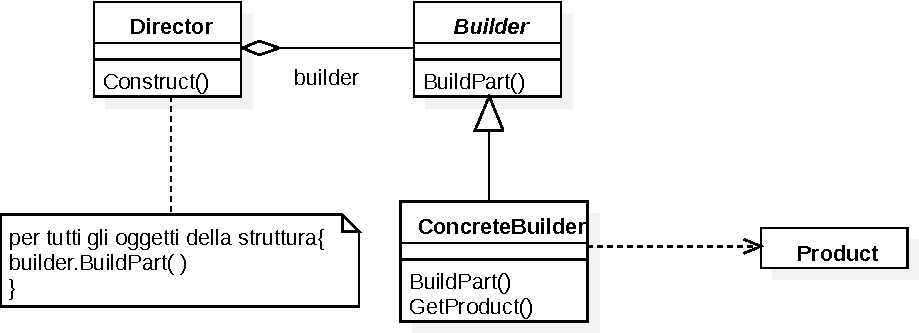
\includegraphics[width=\textwidth,height=\textheight,keepaspectratio]{images/builder-design-pattern.pdf}
\caption{Class diagram di un generico Builder}
\label{fig:builder-design-pattern}
\end{figure}
\subsection{Applicabilità}
Il pattern Builder è solitamente usato nei seguenti casi:
\begin{itemize}
\item l'algoritmo per la creazione di un oggetto deve rimanere separato dalle parti che lo costituiscono e dal modo in cui esse sono composte;
\item il processo di costruzione deve rendere possibili diverse rappresentazioni dell'oggetto a cui è associato.
\end{itemize}
\subsection{Partecipanti}
\begin{itemize}
\item \textbf{Builder} mette a disposizione un interfaccia per la costruzione delle parti dell'oggetto '\textit{Product}'
\item \textbf{ConcreteBuilder} 
	\begin{itemize}
	\item Costruisce le parti dell'oggetto e le assembla secondo una specifica rappresentazione.
	\item Definisce e tiene traccia delle varie rappresentazioni create.
	\item Fornisce un 'interfaccia per ottenere il Product creato.
	\end{itemize}
\item \textbf{Director} sfrutta l'interfaccia del Builder per costruire il Product.
\item \textbf{Product} è l'oggetto complesso che viene costruito. ConcreteBuilder provvede a costruire le sue parti e definisce il processo con cui vengono assemblate. 
\end{itemize}
\subsection{Collaborazioni}
\begin{itemize}
\item Il Client mette in vita il Director e lo configura con il Builder corrispondente alla rappresentazione che desidera costruire.
\item Director manda una richiesta ogni volta che una parte del Product deve essere costruita.
\begin{figure}[htbp]
\centering
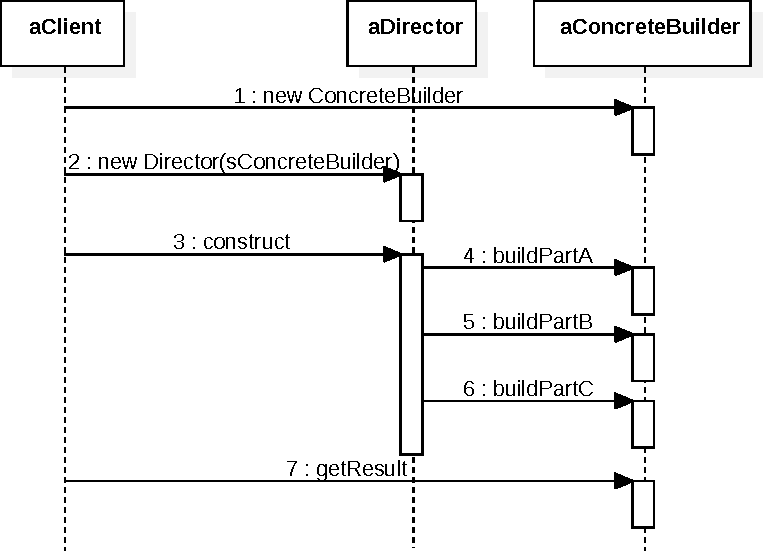
\includegraphics[width=\textwidth,height=\textheight,keepaspectratio]{images/builder-pattern-sequence.pdf}
\caption{Sequence Diagram di un generico Builder}
\label{fig:builder-pattern-sequence}
\end{figure}
\item Builder riceve le richieste del del Director, costruisce e compone le parti del Product
\item Il Client recupera dal Builder il Product costruito.
\end{itemize}

\subsection{Conseguenze}
\begin{enumerate}
\item Consente di variare la rappresentazione interna di un prodotto. Il Builder infatti, grazie alla sua interfaccia, nasconde la struttura interna dell'oggetto che costruisce, quindi per modificarla basta usare una diversa implementazione di questa interfaccia.
\item Migliora la modularizzazione incapsulando il codice necessario alla costruzione dei prodotti. In questo modo i client non hanno bisogno di conoscere la struttura interna dei prodotti. Inoltre Director diversi possono costruire varianti del prodotto con le stesse tipologie di parti interne.
\item Fornisce un controllo sul processo di costruzione molto ravvicinato. Al contrario di altri pattern creazionali che restituiscono il prodotto in un 'colpo' solo, questo segue il processo passo per passo rendendolo molto più controllato e sicuro.
\end{enumerate}

\section{Pattern Visitor}
\label{sec:visitor}
Visitor è uno pattern molto utile che consente di aggiungere nuove funzionalità alle parti di un oggetto composito senza modificare gli oggetti stessi.
\begin{figure}[htbp]
\centering
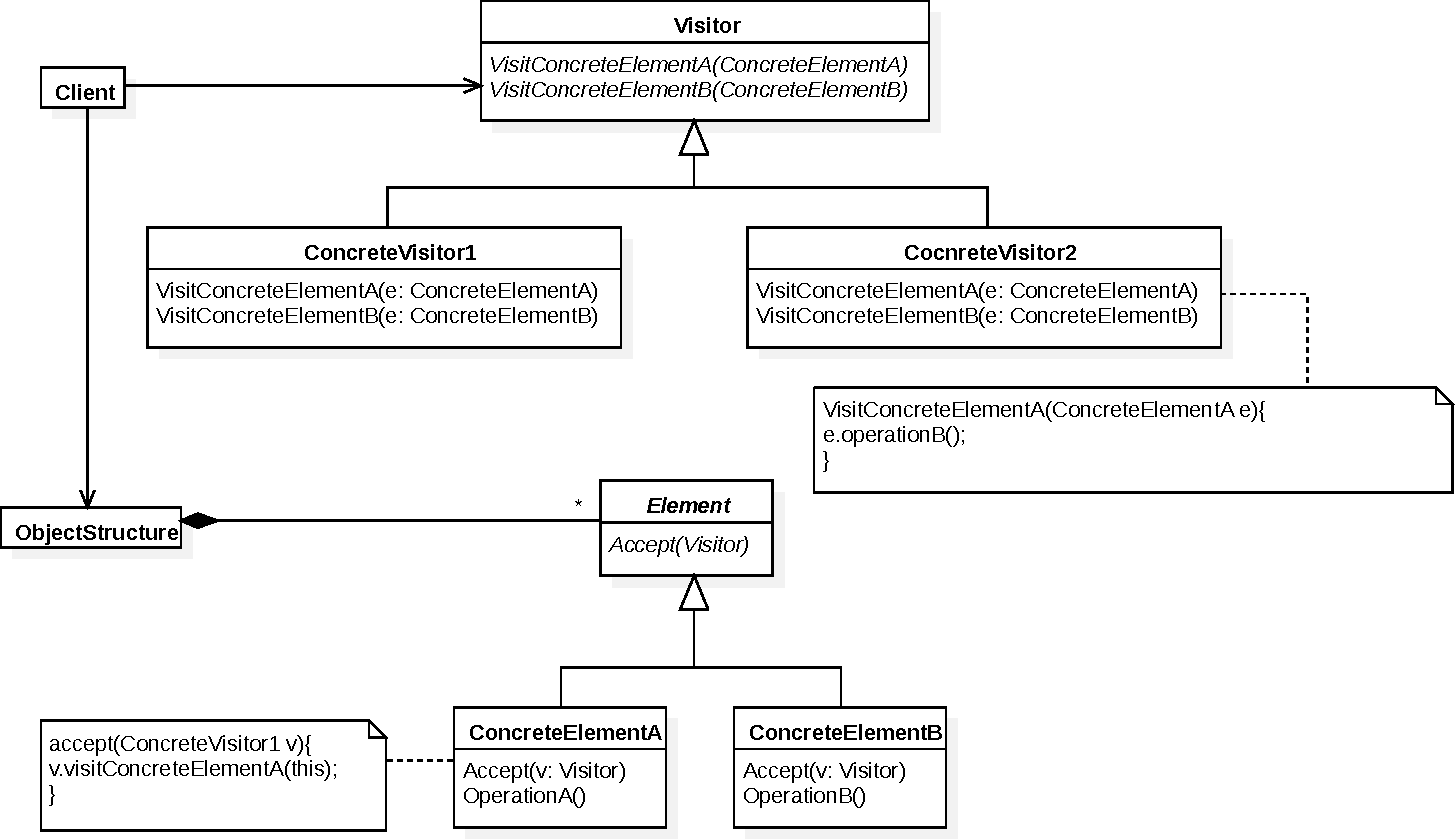
\includegraphics[width=\textwidth,height=\textheight,keepaspectratio]{images/visitor-design-pattern.pdf}
\caption{Class Diagram di un generico Visitor}
\label{fig:visitor-design-pattern}
\end{figure}

\subsection{Applicabilità}
\begin{itemize}
\item Quando si devono eseguire operazioni diversificati in base alla classe concreta degli oggetti che compongono una struttura, ma questi presentano interfacce diverse.
\item Quando devono essere aggiunte operazioni su alcuni oggetti evitando di inquinar le loro interfacce.
\item Quando si ha un frequente bisogno di aggiungere funzionalità a classi che invece cambiano di rado. Infatti nel caso in cui queste classi dovessero cambiare, di dovrebbero modificare e aggiornare tutti i Visitor ad esse associati.
\end{itemize}

\subsection{Partecipanti}
\begin{itemize}
\item \textbf{Visitor} definisce un metodo per ogni ConcreteElement, in modo tale da essere in grado di capire il tipo concreto dell'oggetto che ha chiamato il metodo.
\item \textbf{ConcreteVisitor} implementa tutti i metodi definiti da Visitor. Fornisce inoltre un contesto per l'algoritmo a cui è associato tenendo memoria di eventuali risultati parziali.
\item \textbf{Element} definisce il metodo \texttt{Accept()} con cui viene chiamata l'operazione del Visitor.
\item \textbf{ConcreteElement} implemente il metodo \texttt{Accept()}
\item \textbf{ObjectStructure} può fornire un'interfaccia utile al Visitor per attraversare la struttura.
\end{itemize}

\subsection{Collaborazioni}
\begin{itemize}
\item Il Client crea un oggetto di tipo ConcreteVisitor e attraversa la struttura di oggetti con questo.
\item L'oggetto che viene visitato dal Visitor chiama il metodo per la visita corrispondente alla propria classe concreta passando a se stesso come parametro.
\end{itemize}
\begin{figure}[htbp]
\centering
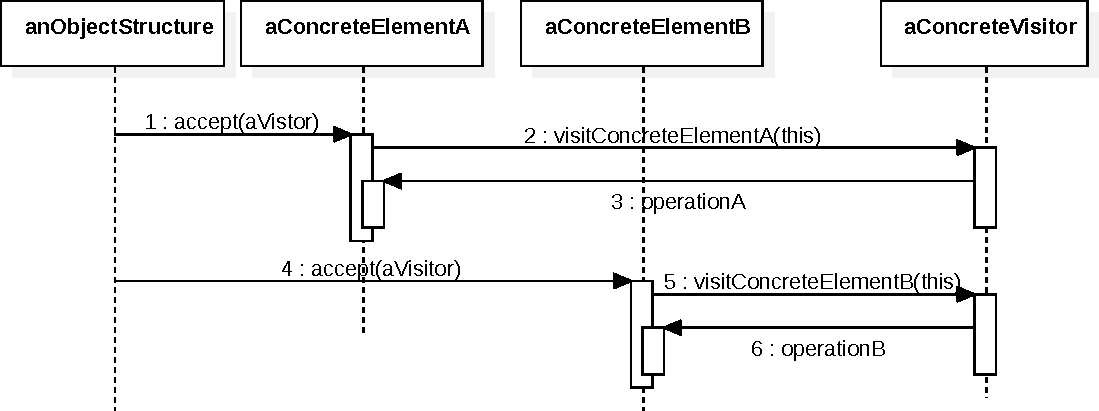
\includegraphics[width=\textwidth,height=\textheight,keepaspectratio]{images/visitor-pattern-sequence.pdf}
\caption{Sequence Diagram di un generico Visitor}
\label{fig:visitor-pattern-sequence}
\end{figure}

\subsection{Conseguenze}
\begin{enumerate}
\item Visitor consente di aggiungere facilmente operazioni a oggetti complessi. Infatti per definire una nuova operazione basterà definire un nuovo Visitor, senza quindi andare a modificare tutte le classi degli oggetti che compongono la struttura nel caso in cui questa operazione coinvolga più di uno di questi oggetti.
\item Aiuta a mantenere le operazioni correlate sotto la stessa classe e a separare quelle scorrelate.
\item Complica l'aggiunta di classi ConcreteElement, poiché questo implica l'aggiornamento di tutte le interfacce dei Visitor che devono poter visitare l'elemento. Quindi è auspicabile usare questo pattern nei casi in cui la struttura rimane invariata o comunque cambia con frequenza minore rispetto alle operazioni da eseguirvi.\\
Nei casi in cui la struttura di classi cambia frequentemente può diventare conveniente aggiungere le operazioni direttamente dentro queste classi.
\item Visitor al contrario di altri pattern come l'\textit{Iterator} non è vincolato a visitare oggetti appartenenti alla stessa classe.
\item Il funzionamento del Visitor è tale da imporre all'elemento concreto di implementare metodi pubblici che accedono al loro stato interno compromettendo quindi il loro incapsulamento.
\item Il Visitor ha il vantaggio di tenere traccia dell'attraversamento della struttura cosa che altrimenti deve essere passa tra i parametri dei vari metodi eseguiti sugli oggetti.
\end{enumerate}


 
